\documentclass[a4paper]{article}

\usepackage[francais,english]{babel}
\usepackage[T1]{fontenc}
\usepackage[]{fullpage}
\usepackage{graphicx}
\usepackage{hyperref}
\usepackage[utf8]{inputenc}
\usepackage{subfigure}

\makeatletter
\def\thickhrulefill{\leavevmode \leaders \hrule height 1pt\hfill \kern \z@}
\def\maketitle{%
  \null
  \thispagestyle{empty}%
  \vskip 1cm
  \begin{flushright}
        \normalfont\Large\@author
  \end{flushright}
  \vfil
  \hrule height 2pt
  \par
  \begin{center}
        \huge \strut \@title \par
  \end{center}
  \hrule height 2pt
  \par
  \vfil
  \vfil
  \null
\begin{center}
\Huge{Placement constraints for a better QoS in clouds}
\end{center}
\begin{figure}[!ht]
	\centering
	\includegraphics[scale=.45]{imgs/cloud.png}
\end{figure}
\vfil
\begin{figure}[!ht]
	\centering
	\includegraphics[scale=.5]{imgs/polytech.png}
\end{figure}
\vfil
\begin{description}
	\item[Entreprise] Université de Nice-Sophia Antipolis
	\item[Lieu] Sophia-Antipolis, France
	\item[Responsable] Fabien Hermenier, équipe OASIS,
		\href{mailto:fabien.hermenier@unice.fr}{fabien.hermenier@unice.fr}
\end{description}
\cleardoublepage
}
\makeatother
\author{Mathieu Bivert, CSSR, \href{mailto:bivert@essi.fr}{bivert@essi.fr}}
\title{PFE: Cahier des charges (DOW)}

\begin{document}
\maketitle

\section{Vocabulaire et notations}
\begin{description}
	\item[Type] entier $t$ associé à chaque système de virtualisation;
	\item[VM] machine virtuelle, notée $v \in \mathcal V$, à laquelle
		est associée un type fixe $T(v)$ et une place $P(v)$;
	\item[Nœud] serveur physique, noté $n \in \mathcal N$,doté d'un
		type courant $T(n)$ et d'un ensemble de types possibles
		$\mathcal{T}_n$;
\end{description}

La fonction $T$ associe à une VM ou un nœud son type; la fonction $P$
associe à une VM un nœud.

Le type d'un nœud est considéré	 comme une dimension, au même titre
que la capacité calculatoire et la mémoire disponible. Cette dimension
est booléenne : soit le type change, auquel cas, la valeur est de $1$,
sinon, elle vaut $0$. Dans les graphes suivants, elle est représentée
à part pour des questions de lisibilité.

\section{Configuration d'exemple}
\subsection{Cas général}
Dans un premier temps, on cherche à obtenir une configuration minimaliste,
mettant en œuvre suffisamment d'éléments pour représenter le problème:
\begin{figure}[!ht]
	\centering
	\includegraphics[scale=.45]{imgs/config.eps}
	\caption{\label{config} Exemple de configuration mettant en œuvre un
		changement de type; $v_1$ est mise hors-ligne, $v_2$ est allumée}
\end{figure}

Sur la figure \ref{config}, $v_1$ et $v_2$ sont deux machines
virtuelles de types différents, par exemple Xen et VMWare.
Pour simplifier le problème, on ne considère que des actions
de démarrage et d'éteignage pour les VMs. En effet, on pourrait
remplacer celles-ci par des migrations par exemple, mais cela
nécessiterait de mettre en ligne d'autres nœuds.

L'opération de déploiement sur le nœud $n_1$ se résume à:
\begin{enumerate}
	\item éteindre $n_1$;
	\item allumer $n_1$ en changeant son type, c'est-à-dire en changeant
		son hyperviseur.
\end{enumerate}
Le temps $T_d$ pris par cette opération est spécifié par l'admninistrateur
du datacenter.

Pour que la reconfiguration puisse avoir lieu, les contraintes suivantes
doivent être respectées:
\begin{itemize}
	\item L'opération de déploiement ne peut commencer que lorsque
		l'utilisation mémoire de $n_1$ est nulle, ie. lorsqu'aucune VM
		ne tourne dessus;
	\item $d_0^{st} \geq c^{ed}$;
	\item $d_1^{st} \geq T_d$;
\end{itemize}

\subsection{Sans changement de type}
On observe maintenant ce qu'il se passe si le type reste constant, de
façon à s'assurer que l'ajout d'une nouvelle dimension ne soit pas
problématique:
\begin{figure}[!ht]
	\centering
	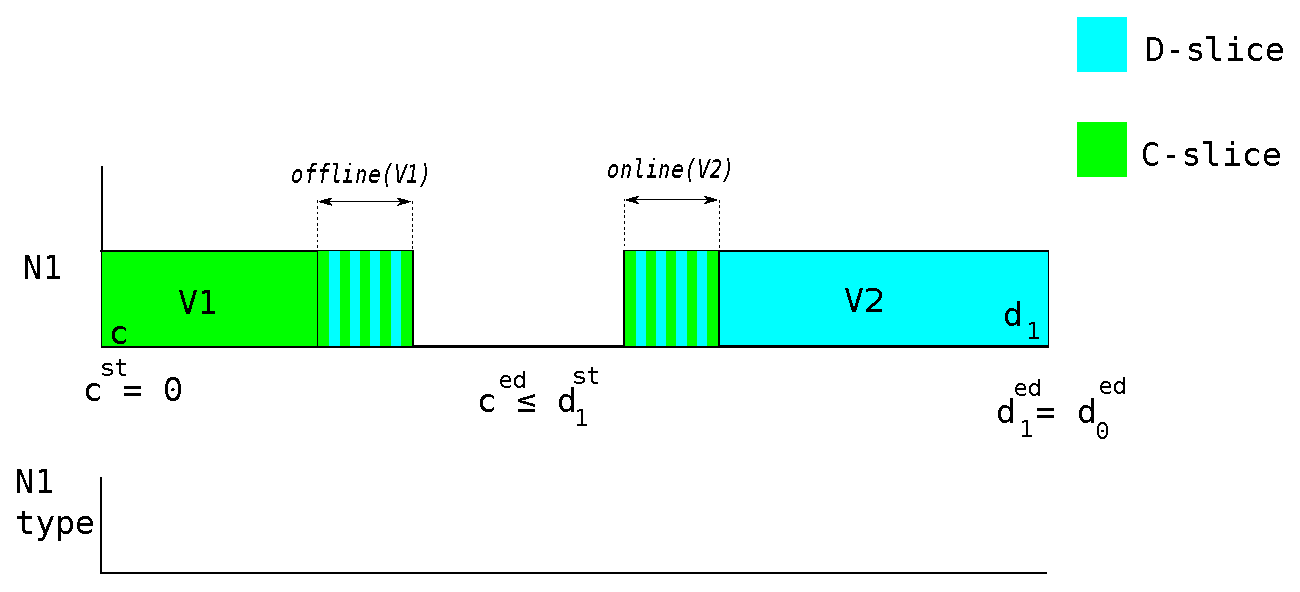
\includegraphics[scale=.45]{imgs/config2.eps}
	\caption{\label{config} Exemple de configuration mettant en œuvre un
		changement de type; $v_1$ est mise hors-ligne, $v_2$ est allumée}
\end{figure}


% \section{Formalisation}
% Le placement est satisfait ssi chaque VM est bien placée sur
% un nœud de même type, ie.:
% \[
% 	(\forall v \in \mathcal V), (\exists n \in \mathcal N), P(v) = n
% 		\Rightarrow T(n) = T(v)	
% \]
% 
% L'un des cas possible pour satisfaire cette condition et de changer le
% type courant d'une machine virtuelle. Une action de déploiement doit
% alors être mise en place.
% 
% La modélisation d'actions de reconfiguration est définie dans ~\cite{herm2012}.
% Elles sont réalisées à l'aide de \textit{slices}, qui correspondent à
% une durée finie pendant un processus de reconfiguration, durant laquelle
% des ressources sont utilisées.
% On distingue plusieurs types de slices:
% \begin{description}
% 	\item[consuming slice], $c \in \mathcal C$, où les ressources sont
% 		utilisées au début de la reconfiguration;
% 	\item[demanding slice], $d \in \mathcal D$, où les ressources sont
% 		utilisées à la fin de la reconfiguration;
% 	\item[middle slice], $m \in \mathcal M$, où les ressources sont utilisées
% 		entre le début et la fin du processus (XXX ambigüe, notation).
% \end{description}
% 
% L'opération de déploiement peut s'exprimer en fonction de ces slices:
% \begin{enumerate}
% 	\item l'état initial (c-slice) lors de la reconfiguration contient les
% 		VMs de l'ancien type devant être déplacées sur un autre serveur ;
% 	\item l'état intermédiaire (m-slice) représente le changement de type,
% 		c'est-à-dire le changement de système de virtualisation. Il
% 		peut être vu comme consommant toutes les ressources disponibles
% 		sur le nœud;
% 	\item l'état final (d-slice) où les VMs du nouveau type sont migrées sur
% 		le nœud.
% \end{enumerate}

\newpage
\selectlanguage{francais}
\bibliographystyle{alpha}
\bibliography{docs}

\end{document}